\begin{figure}[htpb]
        \centering
    \begin{subfigure}{\textwidth}
        \centering
        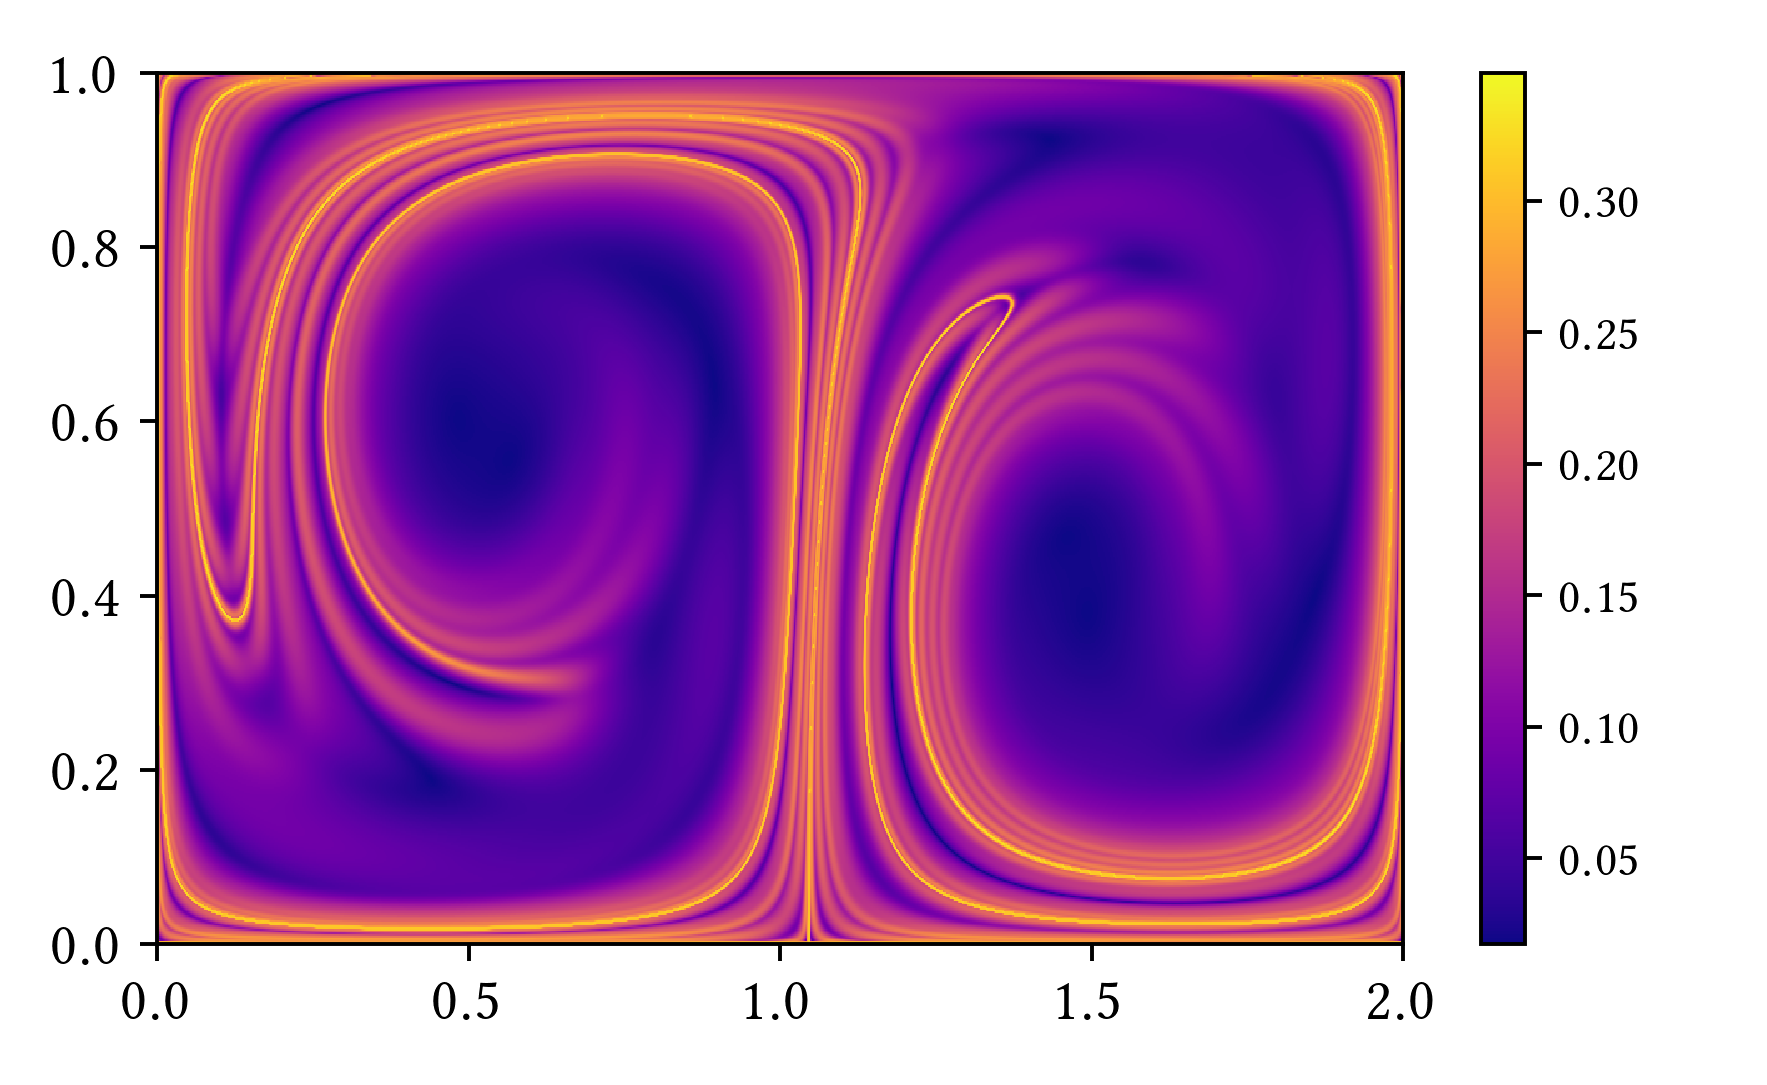
\includegraphics{figures/ftle_l2/ftle.png}
        \caption[]{FTLE field}
%        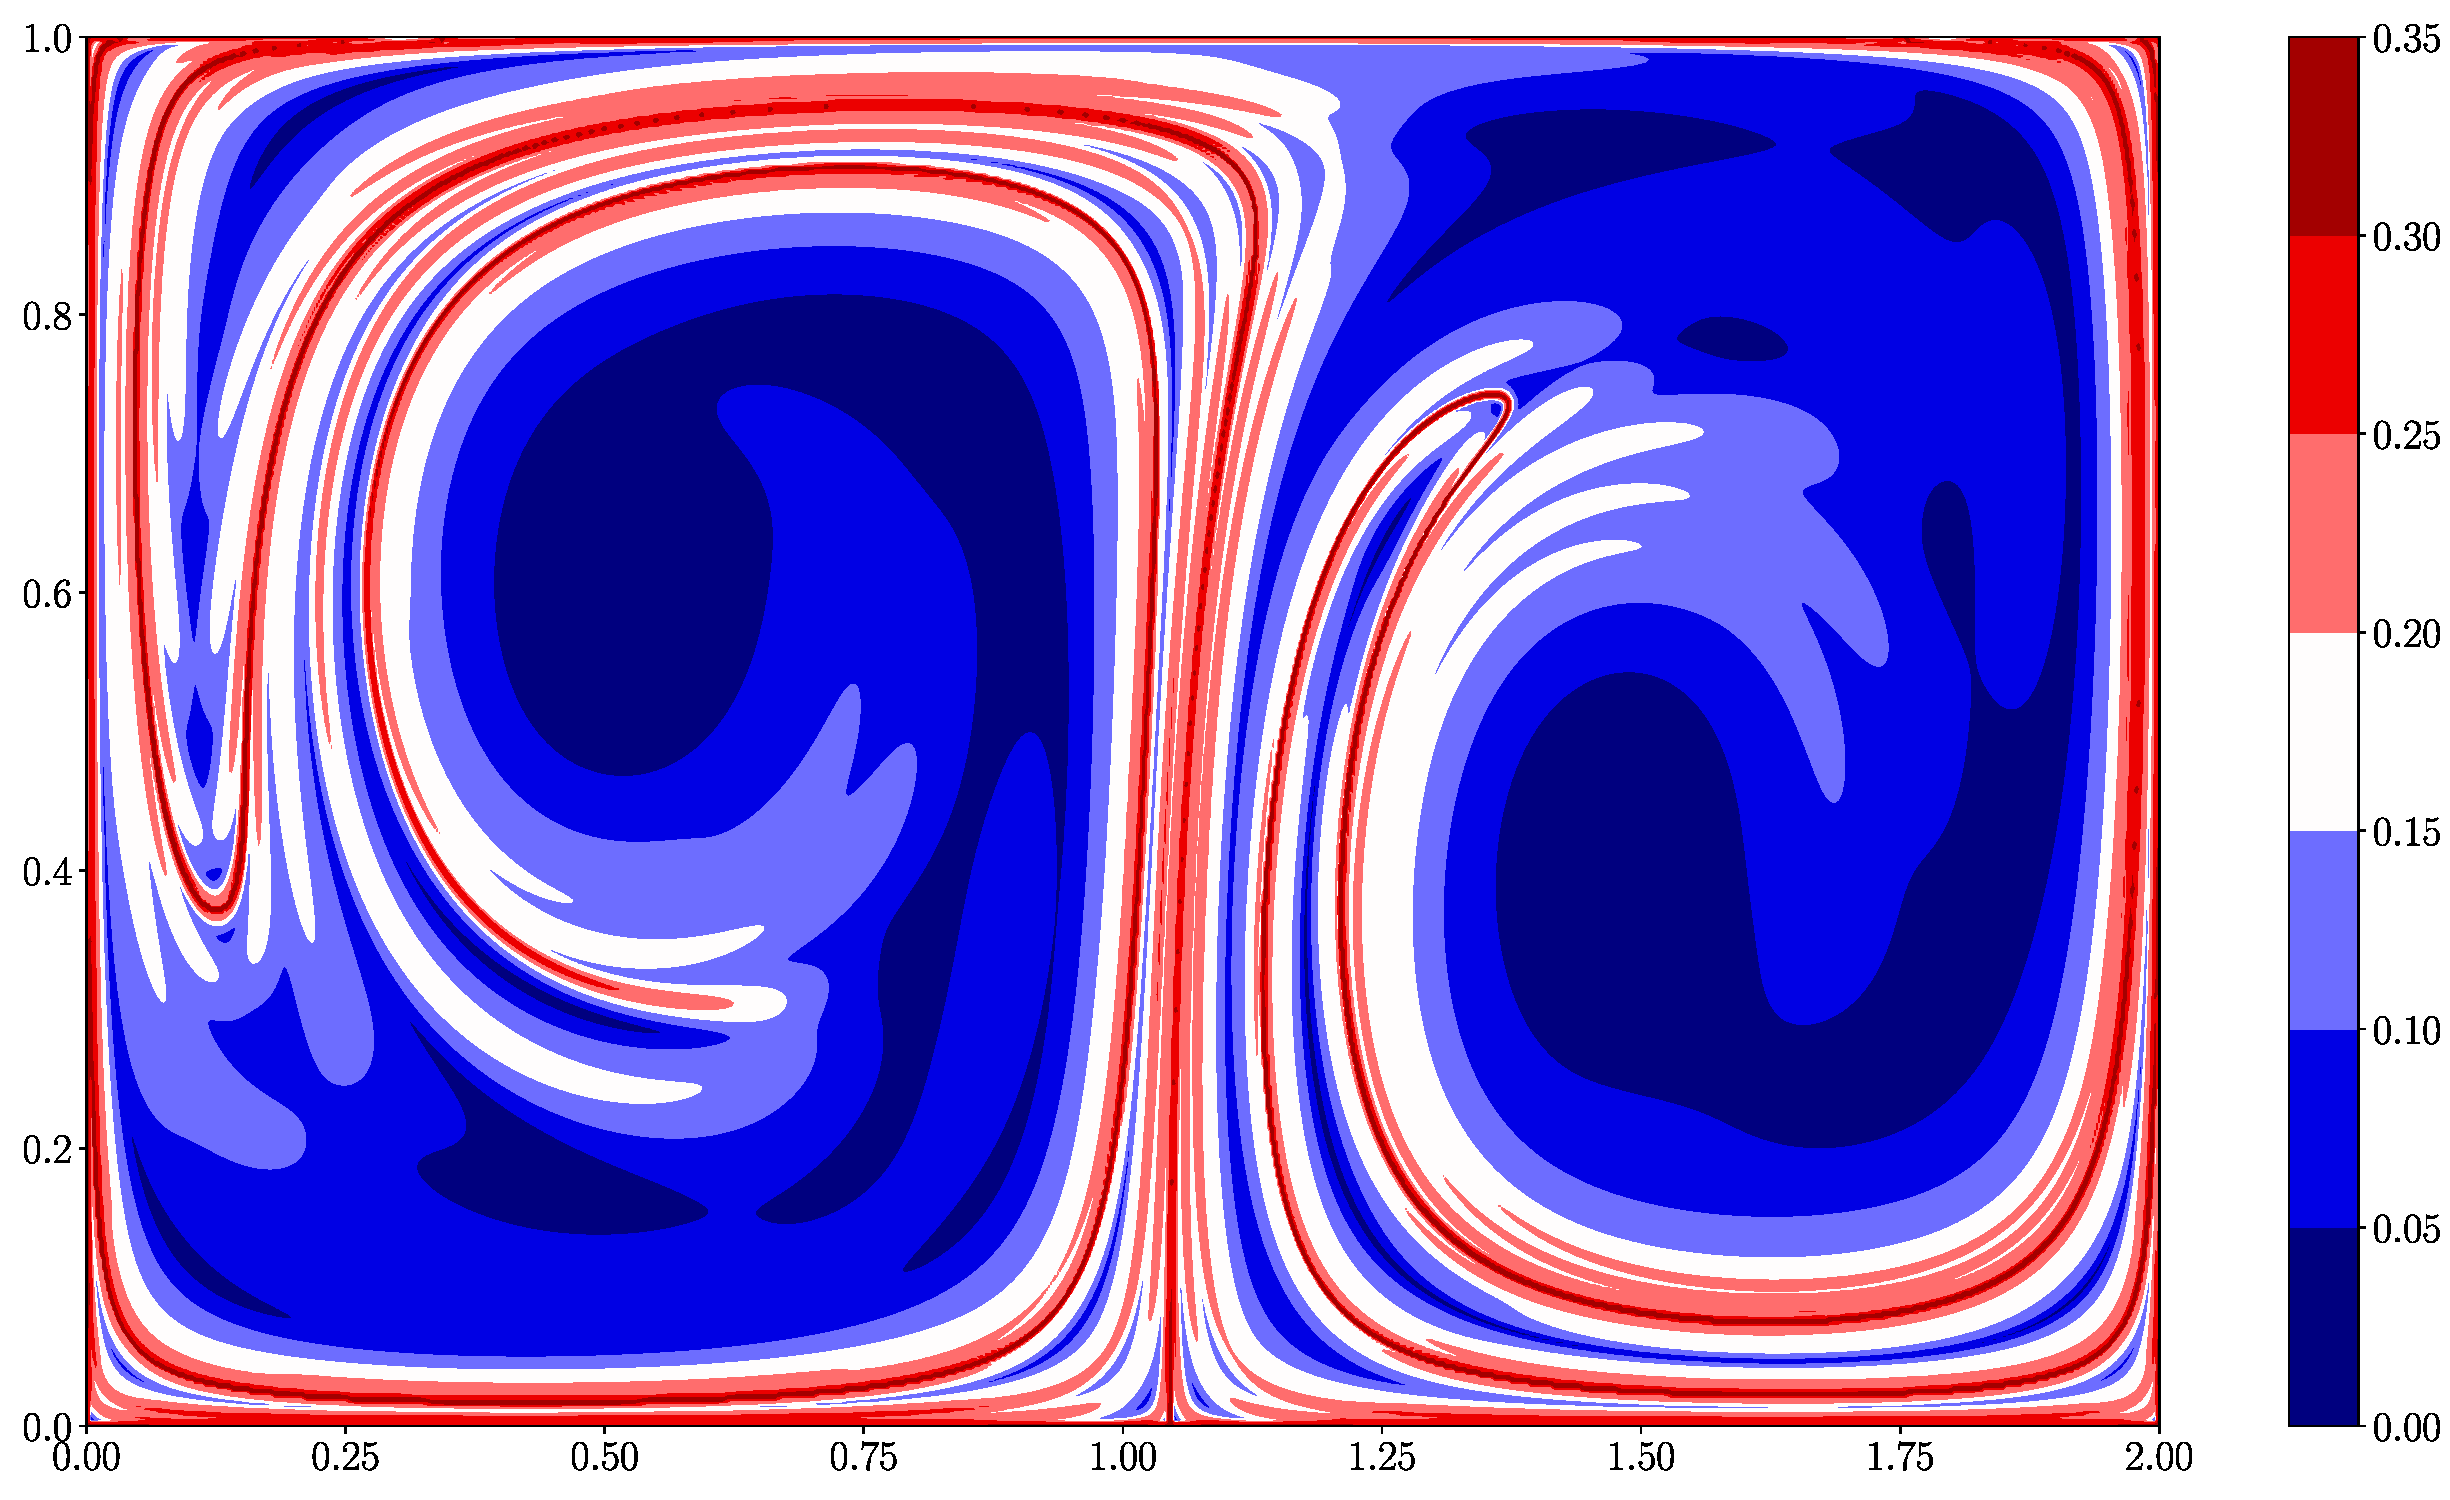
\includegraphics[width=0.75\linewidth,keepaspectratio]{figures/ftle.pdf}
        \label{fig:ftle_l2_ftle}
    \end{subfigure}

    \begin{subfigure}{\textwidth}
        \centering
        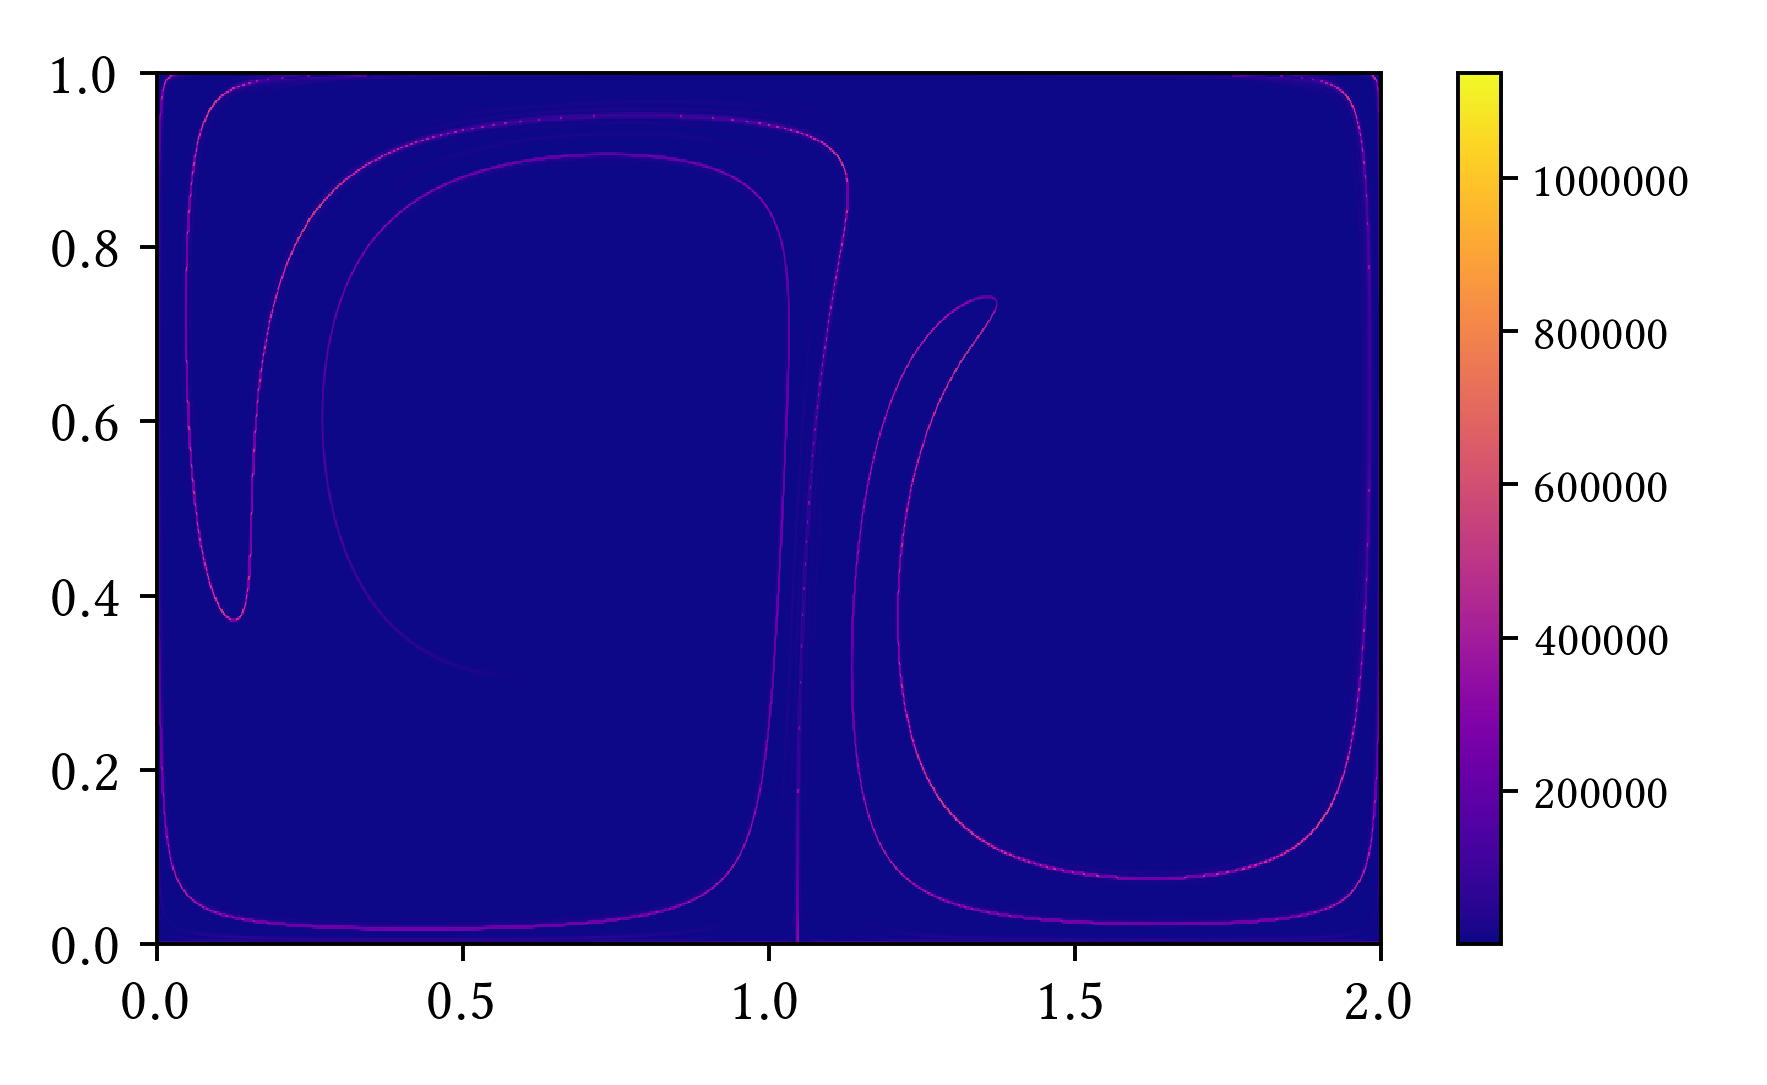
\includegraphics{figures/ftle_l2/l2.png}
        \caption[]{$\lambda_{2}(\vct{x}_{0})$ distribution}
        \label{fig:ftle_l2_l2}
%        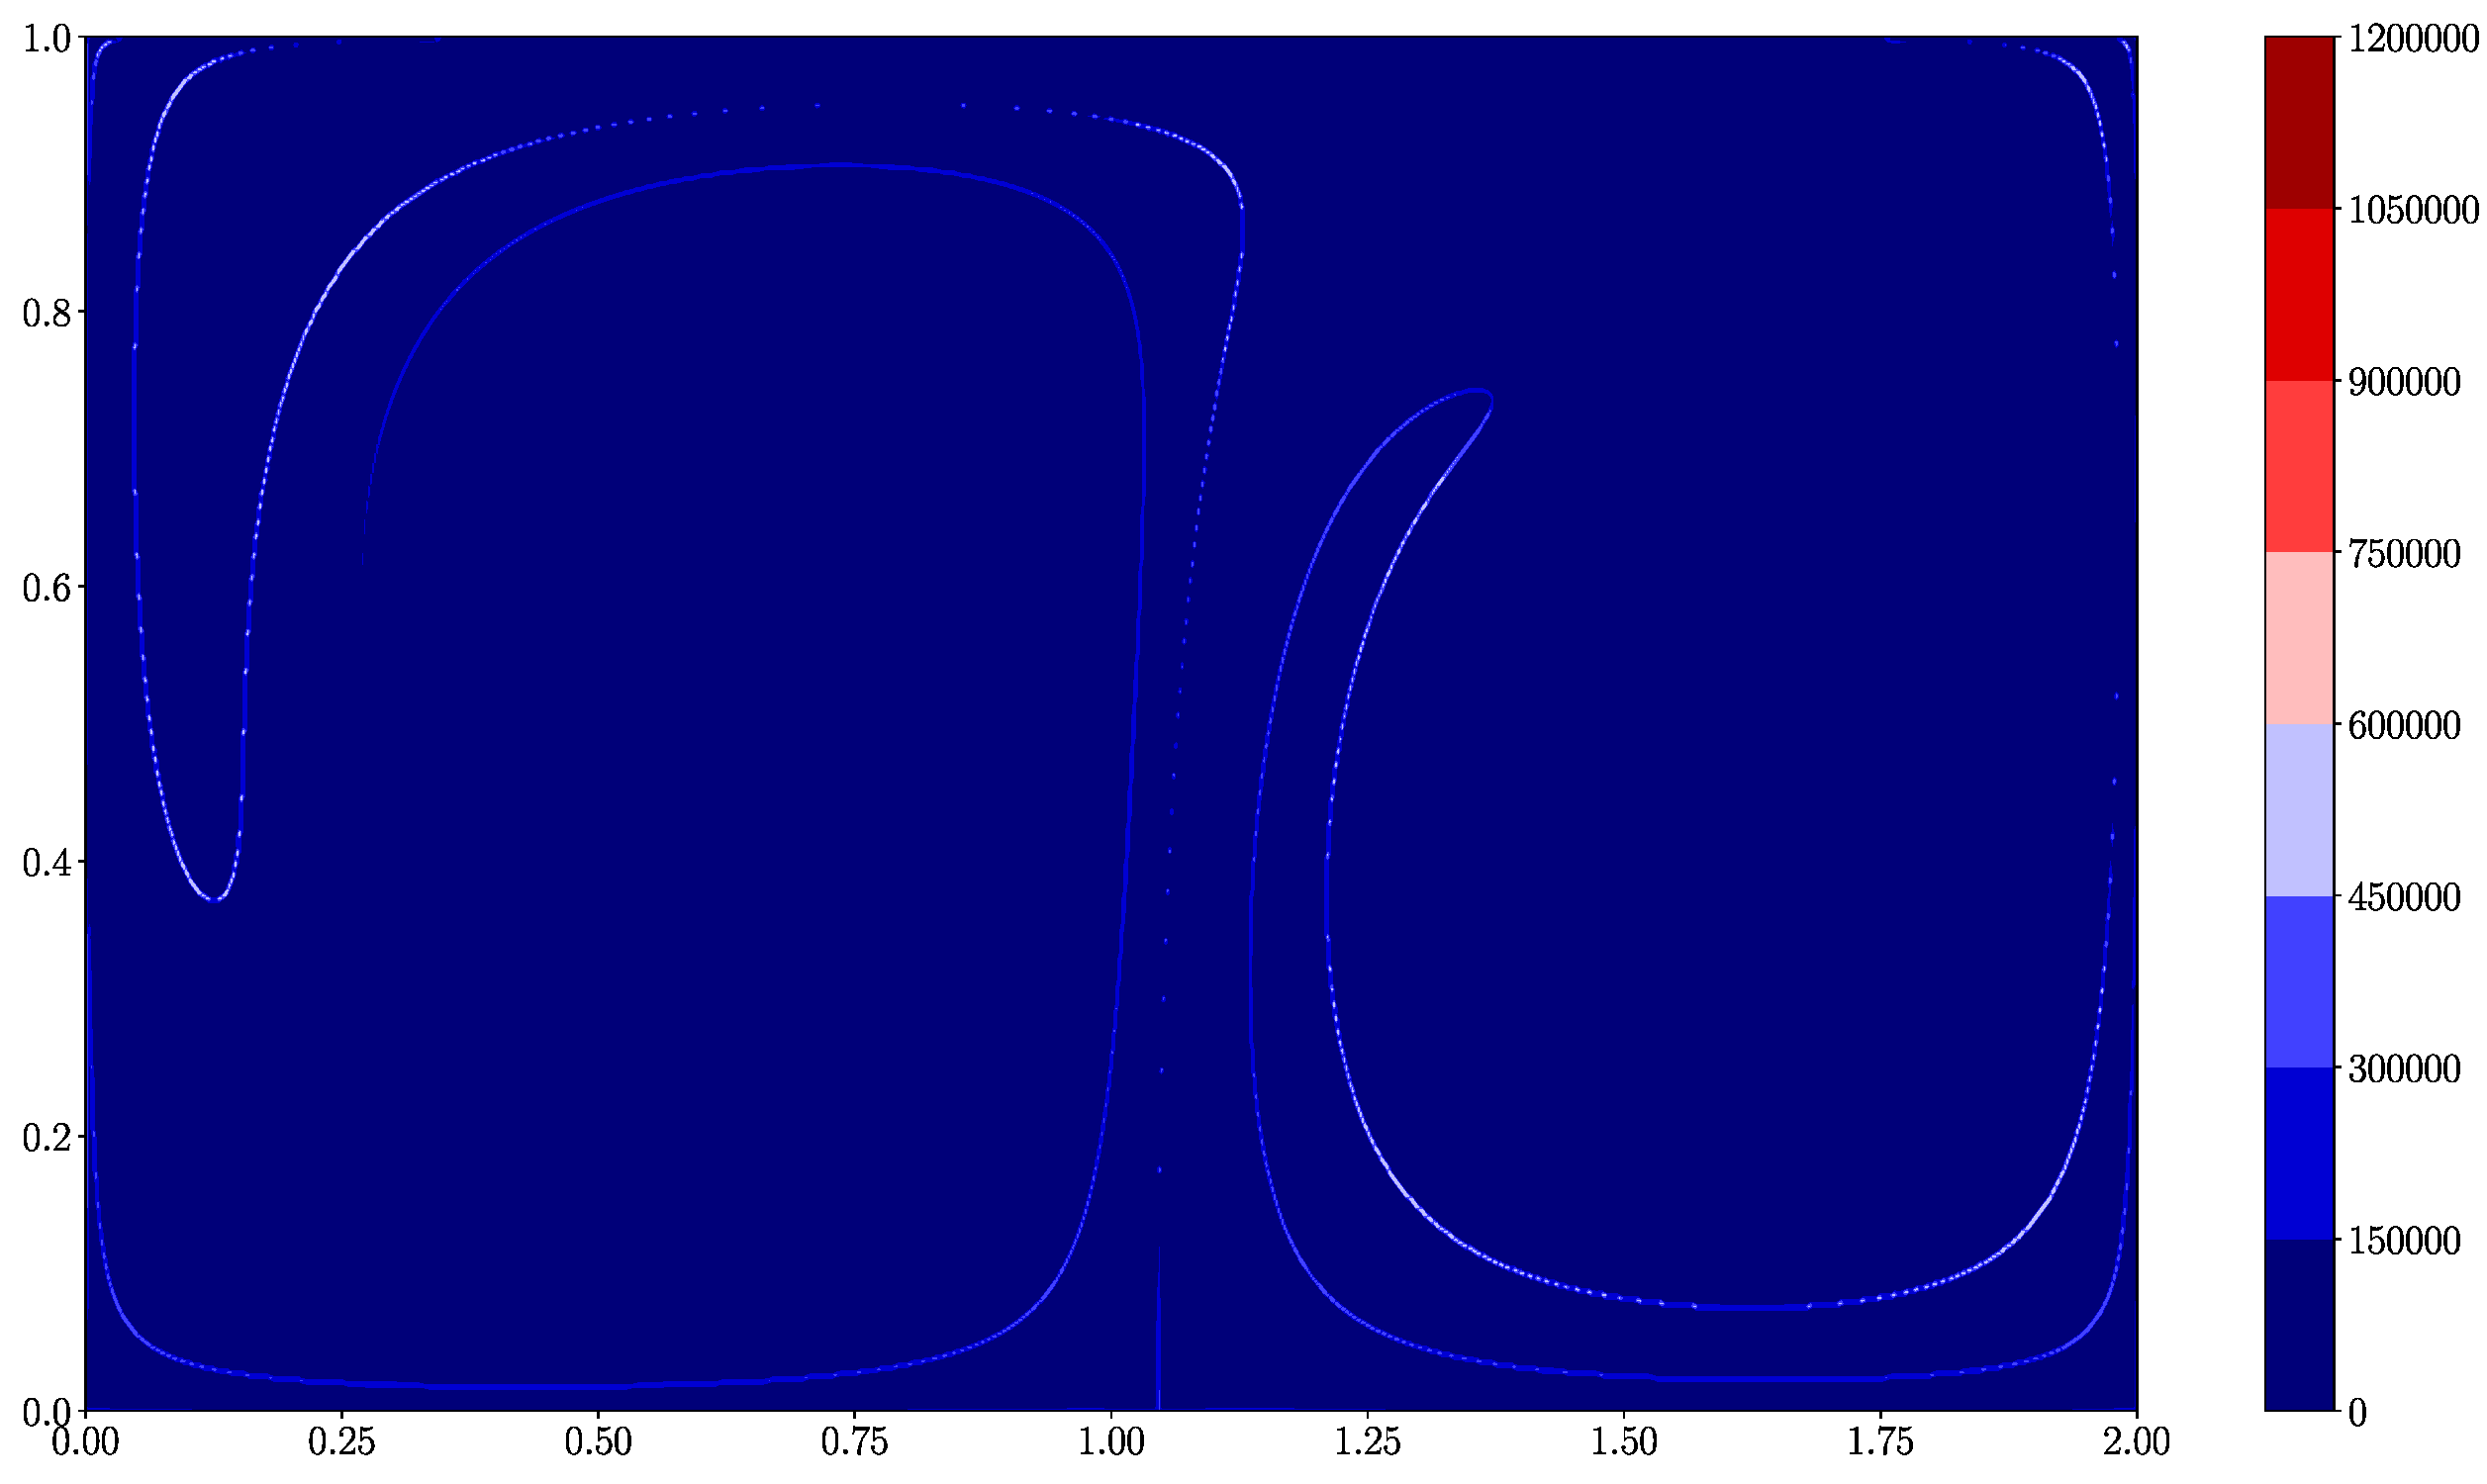
\includegraphics[width=0.75\linewidth,keepaspectratio]{figures/lambda2.pdf}
    \end{subfigure}
    \caption[Plots of the FTLE field and  $\lambda_{2}(\vct{x}_{0})$
    distribution of the double gyre system]{Plots of the FTLE field
    {(\subref{fig:ftle_l2_ftle})} and $\lambda_{2}(\vct{x}_{0})$ distribution
    {(\subref{fig:ftle_l2_l2})} of the double gyre system, defined by
    \cref{eq:doublegyre,eq:doublegyrefuns,eq:doublegyreparams}. Due to the
    different scalings, different levels of detail are resolved. Most notably,
    the $\lambda_{2}(\vct{x}_{0})$ contains a thin, patchy ridge of extremal
    values, whereas a similar, albeit continuous structure is recognizable in
    the FTLE field. Moreover, the FTLE field exhibits a greater amount of detail
    away from the most prominent ridge than the $\lambda_{2}(\vct{x}_{0})$
    distribution. Both plots were used, together with the domain
    $\mathcal{U}_{0}$ shown in \cref{fig:u0_domain}, in order to select
    the lines in $\mathcal{L}$, used to identify local strain maximizing
    strainlines (illustrated in figure~\ref{fig:neighborlcs}).
    }
    \label{fig:ftle_l2}
\end{figure}
